\chapter{Optical Fibers \& Waveguide Theory}



\section{Section 1: Fiber Classification \& Index Profiles [10M] [Priority: High]}

Optical fibers are categorized according to their refractive index profiles and the number of electromagnetic modes they propagate.

\subsection{1. Step-Index (SI) vs. Graded-Index (GI) Fibers}

\begin{itemize}
  \item   \textbf{Step-Index (SI) Fiber:} The core has a uniform refractive index ($n_1$) throughout, which drops abruptly (in a "step") to a lower cladding refractive index ($n_2$) at the core-cladding boundary.
  \item   \textbf{Graded-Index (GI) Fiber:} The refractive index of the core decreases continuously in a parabolic profile from the center ($n_1$) out to the cladding boundary ($n_2$). The profile is governed by:
\end{itemize}
    \[ n(r) = \begin{cases} n_1 \sqrt{1 - 2\Delta\left(\frac{r}{a}\right)^\alpha} & \text{for } r < a \\ n_2 = n_1 \sqrt{1 - 2\Delta} & \text{for } r \ge a \end{cases} \]
    where $a$ is the core radius, $\alpha$ is the profile parameter ($\alpha \approx 2$ for a parabolic profile), and $r$ is the radial distance.

\begin{figure}[H]
\centering
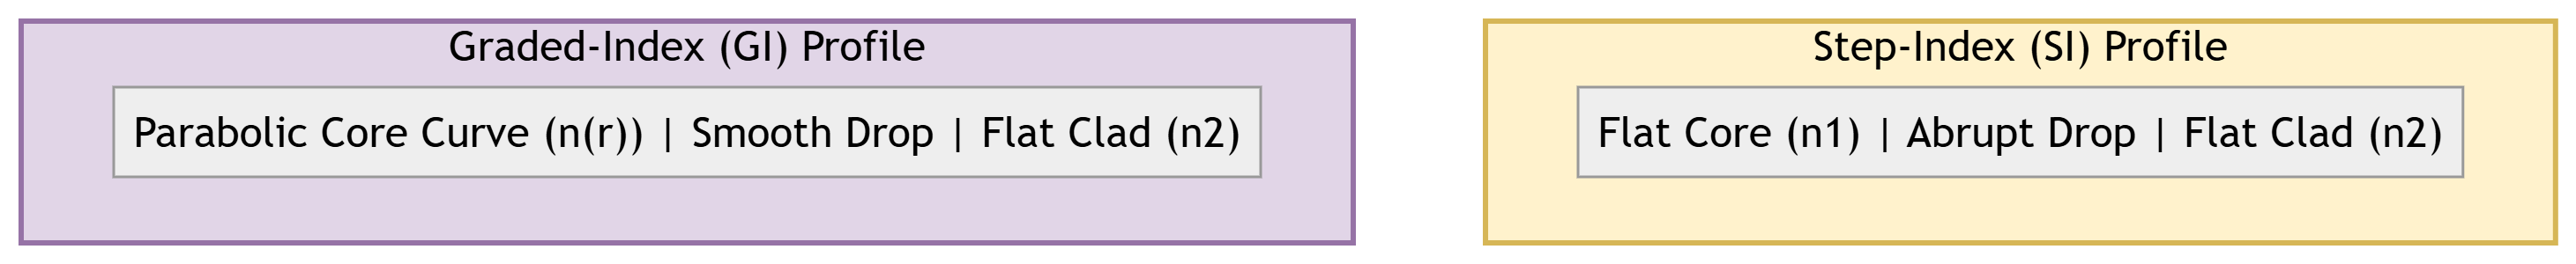
\includegraphics[width=0.75\textwidth,height=0.32\textheight,keepaspectratio]{../Images/chapter_02/index_profiles.png}
\caption{Refractive Index Profiles}
\end{figure}

\begin{table}[H]
\centering
\begin{tabular}{|p{\dimexpr 0.2\textwidth - 2\tabcolsep - 1.5\arrayrulewidth\relax}|p{\dimexpr 0.4\textwidth - 2\tabcolsep - 1.5\arrayrulewidth\relax}|p{\dimexpr 0.4\textwidth - 2\tabcolsep - 1.5\arrayrulewidth\relax}|}
\hline
Feature / Criteria & Step-Index (SI) Fiber & Graded-Index (GI) Fiber \\
\hline
\textbf{Index Profile} & Abrupt step at core-cladding boundary. & Continuous, parabolic decrease from center. \\
\hline
\textbf{Light Propagation} & Zig-zag paths via discrete reflections (TIR). & Continuous sinusoidal, curving refraction paths. \\
\hline
\textbf{Intermodal Dispersion} & High; rays travel different lengths, causing pulse spread. & Low; helical rays travel faster in outer regions, self-focusing. \\
\hline
\textbf{Bandwidth} & Low (typically \textbf{20 MHz·km} for multimode). & High (typically \textbf{2 GHz·km} for multimode). \\
\hline
\textbf{Numerical Aperture} & Constant across the core: $\text{NA} = \sqrt{n_1^2 - n_2^2}$. & Maximum at axis, decreases to zero at cladding boundary. \\
\hline
\textbf{Source Coupling} & Easy; large core and constant NA. & Moderately difficult; requires precise alignment. \\
\hline
\end{tabular}
\end{table}


\subsection{2. Single-Mode (SMF) vs. Multimode (MMF) Fibers}

\begin{itemize}
  \item   \textbf{Single-Mode Fiber (SMF):} Has a small core diameter ($8\text{--}10\ \mu\text{m}$) which permits only the fundamental mode ($\text{HE}_{11}$) to propagate at the operating wavelength.
  \item   \textbf{Multimode Fiber (MMF):} Has a larger core diameter ($50\text{--}100\ \mu\text{m}$) which allows many hundreds of different electromagnetic modes to propagate simultaneously.
\end{itemize}

\begin{table}[H]
\centering
\begin{tabular}{|p{\dimexpr 0.2\textwidth - 2\tabcolsep - 1.5\arrayrulewidth\relax}|p{\dimexpr 0.4\textwidth - 2\tabcolsep - 1.5\arrayrulewidth\relax}|p{\dimexpr 0.4\textwidth - 2\tabcolsep - 1.5\arrayrulewidth\relax}|}
\hline
Feature / Criteria & Single-Mode Fiber (SMF) & Multimode Fiber (MMF) \\
\hline
\textbf{Core Diameter} & Very small ($8\text{--}10\ \mu\text{m}$). & Large ($50\text{--}100\ \mu\text{m}$). \\
\hline
\textbf{Mode Count} & Exactly 1 mode ($\text{HE}_{11}$). & Hundreds of modes ($N \gg 100$). \\
\hline
\textbf{Intermodal Dispersion} & Zero (only one mode exists). & High (significant mode delay differences). \\
\hline
\textbf{Compatible Sources} & Laser Diodes (LD) only. & LEDs and Laser Diodes. \\
\hline
\textbf{Attenuation / Losses} & Extremely low ($0.2\ \text{dB/km}$ at 1550 nm). & Moderately high ($1.0\text{--}3.0\ \text{dB/km}$). \\
\hline
\textbf{Applications} & Long-haul telecom, undersea cables. & Short-haul LANs, data centers, building backbones. \\
\hline
\end{tabular}
\end{table}


\section{Section 2: Key Waveguide Parameters [5M] [Priority: High]}

\subsection{1. Normalized Frequency (V-number)}
The \textbf{V-number} is a dimensionless parameter that determines the number of modes supported by a step-index fiber and dictates its wave propagation limits.
\begin{itemize}
  \item   \textbf{Equation:}
\end{itemize}
    \[ V = \frac{2\pi a}{\lambda} \text{NA} = \frac{2\pi a}{\lambda} \sqrt{n_1^2 - n_2^2} \]
    where $a$ is the core radius, and $\lambda$ is the operating wavelength in free space.
\begin{itemize}
  \item   \textbf{Single-Mode Propagation Condition:} A step-index fiber propagates only the fundamental $\text{HE}_{11}$ mode if the V-number is less than the first zero of the Bessel function $J_0$:
\end{itemize}
    \[ V < 2.405 \]
\begin{itemize}
  \item   \textbf{Guided Modes Count ($N$):}
  \item   For Step-Index Multimode Fibers ($V \gg 2.405$):
\end{itemize}
        \[ N_{SI} \approx \frac{V^2}{2} \]
\begin{itemize}
  \item   For Graded-Index Parabolic Fibers ($\alpha = 2$):
\end{itemize}
        \[ N_{GI} \approx \frac{V^2}{4} \]
        \textit{(GI fibers support half the number of modes as SI fibers for the same V-number).}


\subsection{2. Cutoff Wavelength ($\lambda_c$)}
The \textbf{Cutoff Wavelength} is the transition wavelength above which the fiber supports only a single mode ($\text{HE}_{11}$). Below $\lambda_c$, higher-order modes begin to propagate, and the fiber becomes multimode.
\begin{itemize}
  \item   \textbf{Equation:}
\end{itemize}
    \[ \lambda_c = \frac{2\pi a \text{NA}}{V_c} = \frac{2\pi a \sqrt{n_1^2 - n_2^2}}{2.405} \]
    where $V_c = 2.405$ is the single-mode cutoff limit.


\subsection{3. Mode-Field Diameter (MFD)}
In single-mode fibers, the light is not entirely confined within the core; a fraction of the optical power propagates as an evanescent wave inside the cladding. The \textbf{Mode-Field Diameter (MFD)} is a measure of the radial distribution of the optical power of the fundamental mode.
\begin{itemize}
  \item   \textbf{Definition:} The radial distance between the points where the optical power density drops to $1/e^2$ (or electric field strength drops to $1/e$) of its maximum value at the fiber axis.
  \item   \textbf{Marcuse Formula (for Step-Index Fibers):}
\end{itemize}
    \[ \frac{W}{a} \approx 0.65 + 1.619 V^{-1.5} + 2.879 V^{-6} \]
    where $W$ is the mode-field radius ($MFD = 2W$), and $a$ is the core radius.
\begin{itemize}
  \item   \textbf{Significance:} A smaller MFD increases light confinement but makes splice alignment more sensitive and increases susceptibility to nonlinear effects.
\end{itemize}


\section{Section 3: Waveguide Mode Theory \& Modal Analysis [15M] [Priority: High]}

To describe light propagation in fibers of sub-wavelength dimensions, we solve the vector wave equation derived from Maxwell's equations under cylindrical boundary conditions.

\subsection{1. Maxwell's Equations in Cylindrical Coordinates}

\begin{figure}[H]
\centering
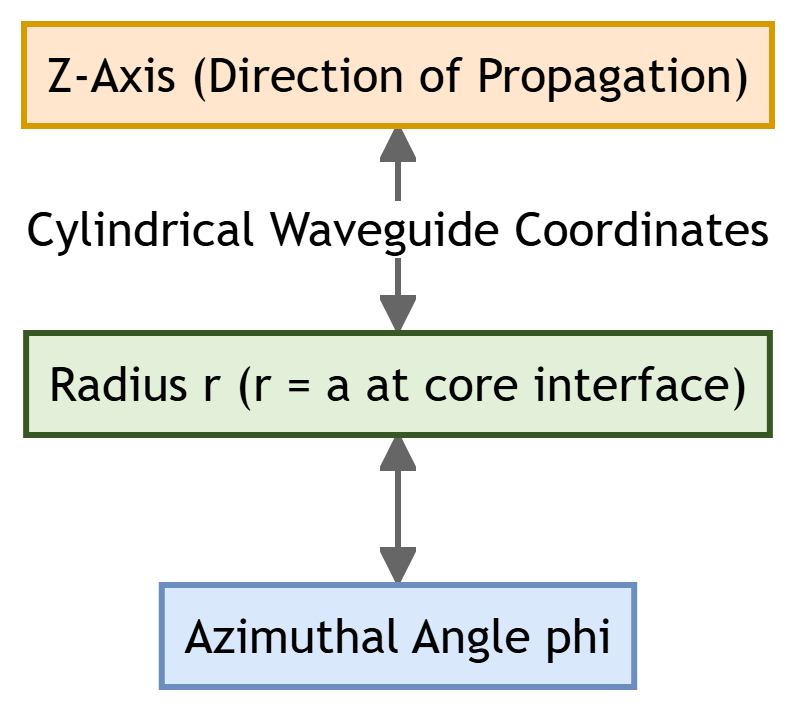
\includegraphics[width=0.75\textwidth,height=0.32\textheight,keepaspectratio]{../Images/chapter_02/cylindrical_coords.png}
\caption{Cylindrical Coordinate Boundaries}
\end{figure}

In cylindrical coordinates $(r, \phi, z)$, assuming waves propagate in the $z$-direction with propagation constant $\beta$ and time-harmonic dependence $e^{j(\omega t - \beta z)}$, the electric ($\vec{E}$) and magnetic ($\vec{H}$) field vectors are:
\[ \vec{E} = \vec{E}_0(r, \phi) e^{j(\omega t - \beta z)}, \quad \vec{H} = \vec{H}_0(r, \phi) e^{j(\omega t - \beta z)} \]

Maxwell's curl equations ($\nabla \times \vec{E} = -j\omega\mu\vec{H}$ and $\nabla \times \vec{H} = j\omega\epsilon\vec{E}$) yield the following component equations:
\begin{enumerate}
  \item $\frac{1}{r}\frac{\partial E_z}{\partial \phi} + j\beta E_\phi = -j\omega\mu H_r$
  \item $-j\beta E_r - \frac{\partial E_z}{\partial r} = -j\omega\mu H_\phi$
  \item $\frac{1}{r}\left[\frac{\partial}{\partial r}(r E_\phi) - \frac{\partial E_r}{\partial \phi}\right] = -j\omega\mu H_z$
  \item $\frac{1}{r}\frac{\partial H_z}{\partial \phi} + j\beta H_\phi = j\omega\epsilon E_r$
  \item $-j\beta H_r - \frac{\partial H_z}{\partial r} = j\omega\epsilon E_\phi$
  \item $\frac{1}{r}\left[\frac{\partial}{\partial r}(r H_\phi) - \frac{\partial H_r}{\partial \phi}\right] = j\omega\epsilon E_z$
\end{enumerate}


\subsection{2. Transverse Fields in Terms of Longitudinal Fields}
By algebraic manipulation of components 1, 2, 4, and 5, the transverse field components ($E_r, E_\phi, H_r, H_\phi$) can be expressed entirely in terms of the longitudinal field components ($E_z, H_z$):
\[ E_r = \frac{-j}{q^2} \left[ \beta \frac{\partial E_z}{\partial r} + \frac{\omega\mu}{r} \frac{\partial H_z}{\partial \phi} \right] \quad \text{--- (Eq 2.1)} \]
\[ E_\phi = \frac{-j}{q^2} \left[ \frac{\beta}{r} \frac{\partial E_z}{\partial \phi} - \omega\mu \frac{\partial H_z}{\partial r} \right] \quad \text{--- (Eq 2.2)} \]
\[ H_r = \frac{-j}{q^2} \left[ \beta \frac{\partial H_z}{\partial r} - \frac{\omega\epsilon}{r} \frac{\partial E_z}{\partial \phi} \right] \quad \text{--- (Eq 2.3)} \]
\[ H_\phi = \frac{-j}{q^2} \left[ \frac{\beta}{r} \frac{\partial H_z}{\partial \phi} + \omega\epsilon \frac{\partial E_z}{\partial r} \right] \quad \text{--- (Eq 2.4)} \]
where $q^2 = k^2 n^2 - \beta^2 = \omega^2\mu\epsilon - \beta^2$.

This reduction simplifies the waveguide analysis to solving a scalar wave equation for $E_z$ and $H_z$ and applying boundary conditions.


\subsection{3. Helmholtz Wave Equation \& Bessel Solutions}
The wave equation for the longitudinal components $E_z$ (and similarly for $H_z$) is:
\[ \frac{\partial^2 E_z}{\partial r^2} + \frac{1}{r}\frac{\partial E_z}{\partial r} + \frac{1}{r^2}\frac{\partial^2 E_z}{\partial \phi^2} + q^2 E_z = 0 \]

Using separation of variables, $E_z(r, \phi) = F(r) e^{j\nu\phi}$ (where $\nu$ is an integer representing azimuthal variation), we obtain the \textbf{Bessel Differential Equation} for the radial function $F(r)$:
\[ \frac{d^2 F}{dr^2} + \frac{1}{r}\frac{dF}{dr} + \left(q^2 - \frac{\nu^2}{r^2}\right) F = 0 \]

\subsubsection{Solutions:}
\begin{enumerate}
  \item \textbf{Core Region ($r < a$, index $n_1$):}
\end{enumerate}
    The transverse parameter is $u^2 = a^2(k_0^2 n_1^2 - \beta^2) > 0$. The solution must remain finite at $r=0$, which requires the \textbf{Bessel function of the first kind ($J_\nu$)}:
    \[ E_z(r, \phi) = A J_\nu\left(\frac{u r}{a}\right) e^{j\nu\phi}, \quad H_z(r, \phi) = B J_\nu\left(\frac{u r}{a}\right) e^{j\nu\phi} \]
\begin{enumerate}
  \item \textbf{Cladding Region ($r > a$, index $n_2$):}
\end{enumerate}
    For guided waves, the fields must decay to zero as $r \to \infty$. The transverse parameter is $w^2 = a^2(\beta^2 - k_0^2 n_2^2) > 0$. The solution requires the \textbf{Modified Bessel function of the second kind ($K_\nu$)}:
    \[ E_z(r, \phi) = C K_\nu\left(\frac{w r}{a}\right) e^{j\nu\phi}, \quad H_z(r, \phi) = D K_\nu\left(\frac{w r}{a}\right) e^{j\nu\phi} \]


\subsection{4. Boundary Conditions \& Eigenvalue Equation}
At the core-cladding interface ($r = a$), the tangential components of the electric and magnetic fields must be continuous:
\[ E_z(a^-) = E_z(a^+), \quad H_z(a^-) = H_z(a^+) \]
\[ E_\phi(a^-) = E_\phi(a^+), \quad H_\phi(a^-) = H_\phi(a^+) \]

Substituting the Bessel solutions for $E_z$ and $H_z$ into Equations 2.2 and 2.4 to find $E_\phi$ and $H_\phi$, and matching them at $r = a$ yields a system of four linear equations for constants $A, B, C$, and $D$. Setting the determinant of this system to zero gives the transcendental \textbf{Characteristic Equation}:
\[ \left[ \frac{J_\nu'(u)}{u J_\nu(u)} + \frac{K_\nu'(w)}{w K_\nu(w)} \right] \left[ \frac{J_\nu'(u)}{u J_\nu(u)} + \frac{n_2^2}{n_1^2} \frac{K_\nu'(w)}{w K_\nu(w)} \right] = \nu^2 \left( \frac{1}{u^2} + \frac{1}{w^2} \right) \left( \frac{1}{u^2} + \frac{n_2^2}{n_1^2} \frac{1}{w^2} \right) \]

\begin{itemize}
  \item   For $\nu = 0$, the right-hand side is zero. The equations decouple, yielding:
  \item   \textbf{TE Modes ($\nu=0, E_z=0$):} $\frac{J_0'(u)}{u J_0(u)} + \frac{K_0'(w)}{w K_0(w)} = 0$
  \item   \textbf{TM Modes ($\nu=0, H_z=0$):} $\frac{J_0'(u)}{u J_0(u)} + \frac{n_2^2}{n_1^2} \frac{K_0'(w)}{w K_0(w)} = 0$
  \item   For $\nu \neq 0$, the fields are coupled, producing hybrid \textbf{HE} and \textbf{EH} modes.
\end{itemize}


\section{Section 4: Practice Problems [10M] [Priority: High]}

\subsection{Problem 2.1: Multimode Step-Index Fiber Characterization}
\textbf{Given:}
\begin{itemize}
  \item   Core diameter ($2a$) = $80\ \mu\text{m} \implies$ core radius ($a$) = $40\ \mu\text{m} = 40 \times 10^{-6}\ \text{m}$
  \item   Core refractive index ($n_1$) = \textbf{1.48}
  \item   Relative refractive index difference ($\Delta$) = $1.5\% = 0.015$
  \item   Operating wavelength ($\lambda$) = $0.85\ \mu\text{m} = 0.85 \times 10^{-6}\ \text{m}$
\end{itemize}

\textbf{Formulas:}
\begin{enumerate}
  \item Numerical Aperture: $\text{NA} = n_1\sqrt{2\Delta}$
  \item Normalized Frequency: $V = \frac{2\pi a}{\lambda}\text{NA}$
  \item Total Guided Modes: $N \approx \frac{V^2}{2}$
\end{enumerate}

\textbf{Step 1: Calculate the Numerical Aperture (NA):}
\[ \text{NA} = 1.48 \times \sqrt{2 \times 0.015} = 1.48 \times \sqrt{0.03} \]
\[ \text{NA} = 1.48 \times 0.1732 = 0.2563 \]

\textbf{Step 2: Calculate the V-number:}
\[ V = \frac{2\pi \times 40 \times 10^{-6}}{0.85 \times 10^{-6}} \times 0.2563 \]
\[ V = \frac{251.327}{0.85} \times 0.2563 \approx 295.68 \times 0.2563 \]
\[ V \approx 75.78 \]

\textbf{Step 3: Calculate the number of guided modes ($N$):}
\[ N = \frac{(75.78)^2}{2} = \frac{5742.6}{2} \approx 2871 \]

\textbf{Final Answer:}
\begin{itemize}
  \item   The Normalized Frequency (V-number) is \textbf{75.78}.
  \item   The total number of guided modes is \textbf{2871}.
\end{itemize}


\subsection{Problem 2.2: Cutoff Wavelength of Single-Mode Fiber}
\textbf{Given:}
\begin{itemize}
  \item   Core radius ($a$) = $4\ \mu\text{m} = 4 \times 10^{-6}\ \text{m}$
  \item   Core refractive index ($n_1$) = \textbf{1.48}
  \item   Relative refractive index difference ($\Delta$) = $0.2\% = 0.002$
  \item   Cutoff V-number ($V_c$) = \textbf{2.405}
\end{itemize}

\textbf{Formulas:}
\begin{enumerate}
  \item Numerical Aperture: $\text{NA} = n_1\sqrt{2\Delta}$
  \item Cutoff Wavelength: $\lambda_c = \frac{2\pi a \text{NA}}{V_c}$
\end{enumerate}

\textbf{Step 1: Calculate the Numerical Aperture (NA):}
\[ \text{NA} = 1.48 \times \sqrt{2 \times 0.002} = 1.48 \times \sqrt{0.004} \]
\[ \text{NA} = 1.48 \times 0.06325 \approx 0.0936 \]

\textbf{Step 2: Calculate the Cutoff Wavelength ($\lambda_c$):}
\[ \lambda_c = \frac{2\pi \times (4 \times 10^{-6}\ \text{m}) \times 0.0936}{2.405} \]
\[ \lambda_c = \frac{2.352 \times 10^{-6}}{2.405}\ \text{m} \]
\[ \lambda_c \approx 0.978 \times 10^{-6}\ \text{m} = 0.978\ \mu\text{m} = 978\ \text{nm} \]

\textbf{Final Answer:}
The cutoff wavelength of the single-mode fiber is \textbf{$0.978\ \mu\text{m}$} (or \textbf{$978\ \text{nm}$}).
